\documentclass{beamer}

\usepackage{amsmath}
\usepackage{amssymb}
\usepackage{graphicx}

\newcommand{\parens}[1]{\left(#1\right)}
\newcommand{\set}[1]{\left\{#1\right\}}

\title{Ordered Line Integral Methods for the Solving the Eikonal Equation}
\author{Samuel F. Potter \and Maria Cameron}

\begin{document}

\frame{\titlepage}

\begin{frame}
  \frametitle{Setup}

  \begin{center}
    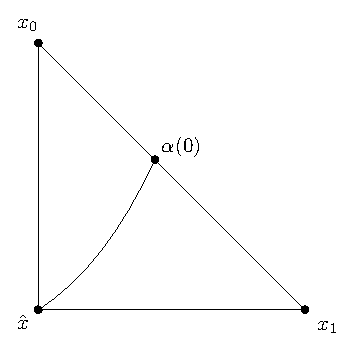
\includegraphics[width=0.35\linewidth]{path.eps}
  \end{center}

  Replace finite differences with local functional minimization
  problems, e.g.:
  \begin{equation*}
    \hat{u} = \min_{\alpha : \alpha(0) \in [x_0, x_1]} \set{u(\alpha(0)) + \int_{\alpha} s(\hat{x} + \alpha(t)) |\alpha'(t)| dt}
  \end{equation*}
\end{frame}

\begin{frame}
  \frametitle{Setup}

  We approximate the characteristic locally with a straight line, and
  explore three different quadrature rules:

  \begin{itemize}
  \item \texttt{rhr}: $u_\lambda + \hat{s} h ||\hat{x} - x_\lambda||$, \hspace{4.4em} $\hat{s} = s(\hat{x})$
  \item \texttt{mp0}: $u_\lambda + \parens{\frac{\hat{s} + \langle s_i \rangle}{2}} h ||\hat{x} - x_\lambda||$, \hspace{1.05em} $\langle s_i \rangle = \tfrac{1}{n} \sum_{i} s(x_i)$
  \item \texttt{mp1}: $u_\lambda + s_\lambda h ||\hat{x} - x_\lambda||$, \hspace{4.0em} $s_\lambda = \sum_i \lambda_i s(x_i)$
  \end{itemize}

  Think of $\texttt{mp0}$ as being a cross between $\texttt{rhr}$ and
  $\texttt{mp1}$.
\end{frame}

\begin{frame}
  More generally, have the point in the rectangle rule to correspond
  to a section in the simplex $\mbox{conv}(\hat{x}, x_0, x_1, x_2)$
  selected using a parameter $\theta \in [0, 1]$
  
  \begin{center}
    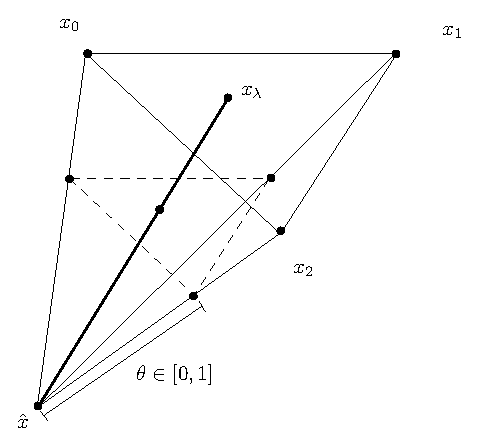
\includegraphics[width=0.6\linewidth]{theta-rule.eps}
  \end{center}
\end{frame}

\begin{frame}
  \frametitle{Minimization}

  We use a projected Newton's method where we parametrize
  $\mbox{conv}(x_0, x_1, x_2)$ by
  $\Delta = \set{(\lambda_1, \lambda_2) : \lambda_i \geq 0,
    \hspace{0.5em} \lambda_1 + \lambda_2 \leq 1}$, which forms the
  constraint set

  \begin{center}
    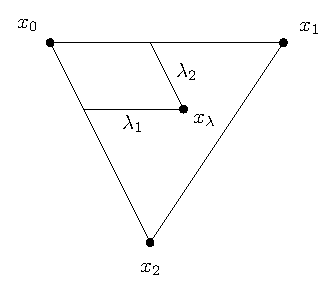
\includegraphics[width=0.5\linewidth]{lambda-coords.eps}
  \end{center}
\end{frame}

\begin{frame}
  \frametitle{Minimization}
  
  Projected Newton's method is extremely efficient for low-dimensional
  problems (converges to machine precision in a few iterations, and
  each iteration is inexpensive)

  \vspace{1em}

  Each step is solved using the active set method for
  inequality-constrained quadratic programming

  \vspace{1em}

  Involves KKT theory which ends up being useful for deciding which
  updates to do
\end{frame}

\begin{frame}
  \frametitle{Minimization}

  Can't use \texttt{mp0} directly, it's inconsistent

  \vspace{1em}

  But \texttt{mp0} is cheaper to minimize than \texttt{mp1} (simpler
  Hessian)

  \vspace{1em}

  Minimizing \texttt{mp0} and then using the minimizing argument to
  evaluate \texttt{mp1} is consistent for a Lipschitz slowness function,
  and appears to only incur $O(h^3)$ error per update
\end{frame}

\begin{frame}
  \frametitle{Update Pruning}

  \begin{center}
    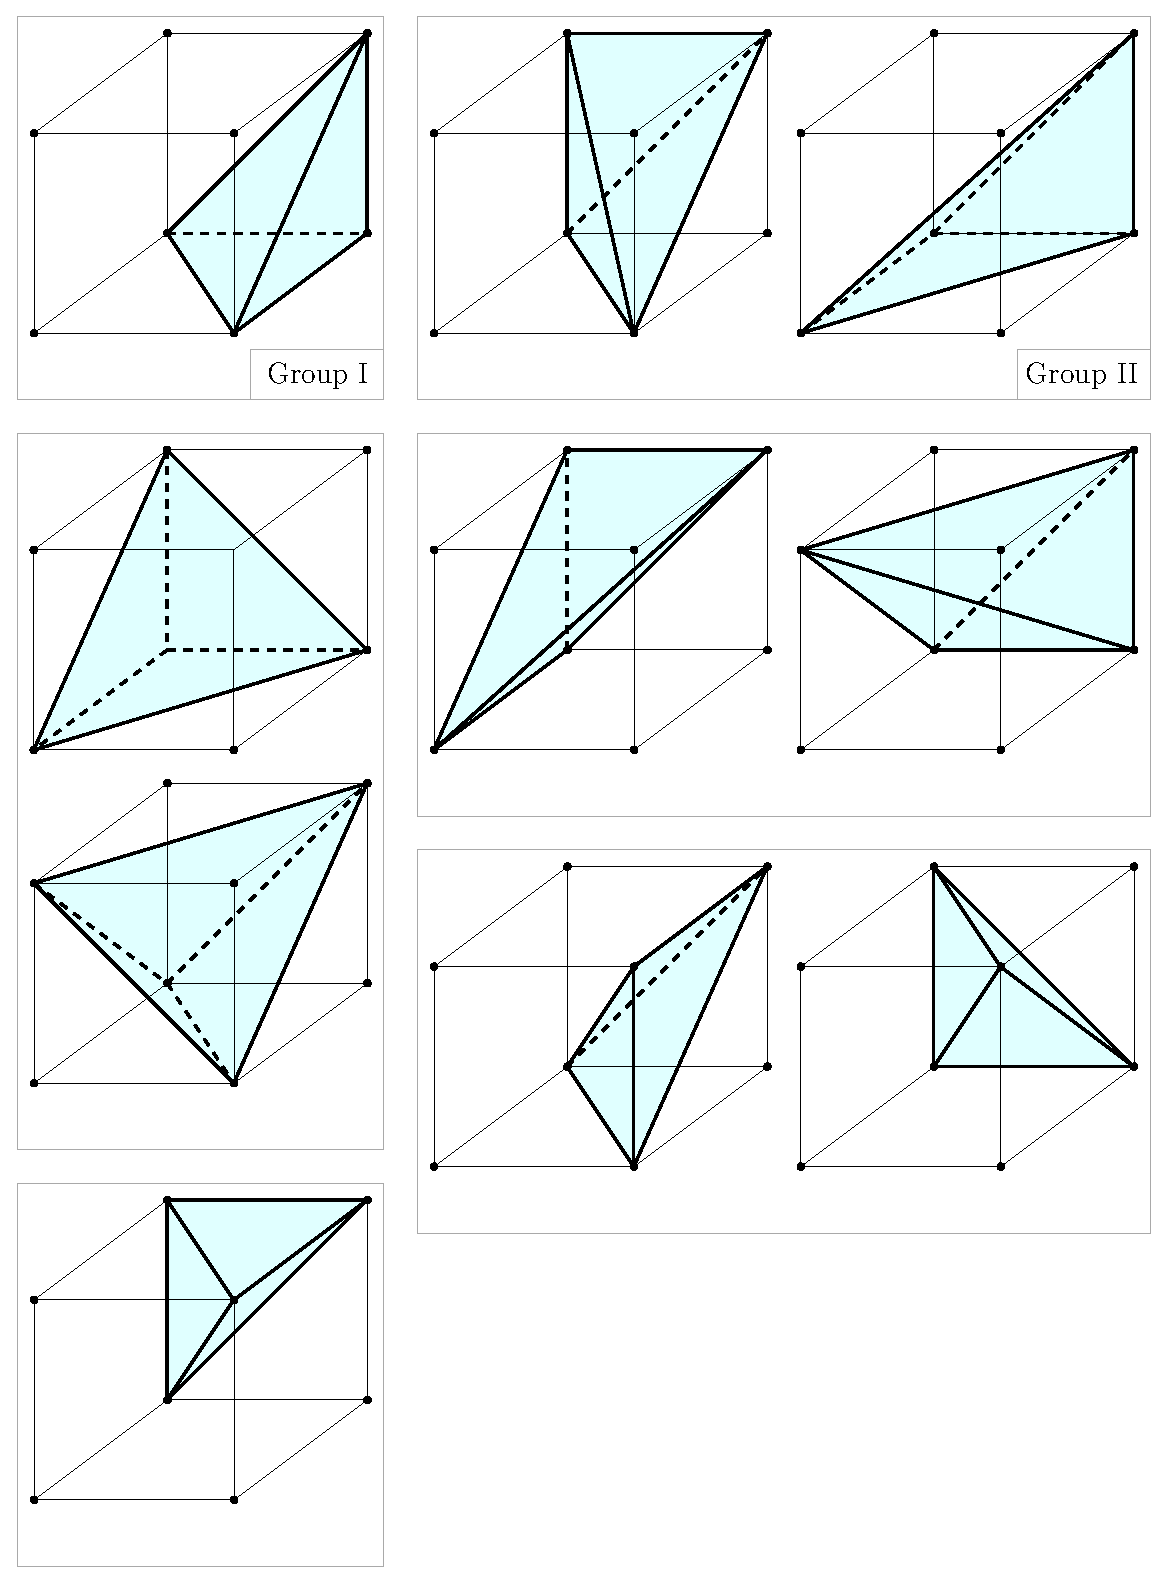
\includegraphics[width=0.56\linewidth]{tetra-by-group.eps}
  \end{center}
\end{frame}

\begin{frame}
  \frametitle{Hierarchical Update}

  A heuristic:
  \begin{itemize}
  \item Find the minimal one-point update\ldots
  \item Find the minimal adjacent two-point update\ldots
  \item Find the minimal adjacent three-point update\dots
  \end{itemize}
  
  \vspace{1em}

  Use KKT theory to rule out updates

  \vspace{1em}

  Establish an error bound for this
\end{frame}

\end{document}

%%% Local Variables:
%%% mode: latex
%%% TeX-master: t
%%% End:
